\documentclass{article}
\usepackage{amsmath}
\usepackage{float}
\usepackage{hyperref}
\usepackage{geometry}
 \geometry{
 a4paper,
 total={170mm,257mm},
 left=20mm,
 top=10mm,
 }

\usepackage{graphicx}
\graphicspath{ {./images/} }

\title{PH456 Lab 2 : Using Random Numbers} % Sets article title
\author{Sourabh Choudhary} % Sets authors name
\date{\today} % Sets date for date compiled

% The preamble ends with the command \begin{document}
\begin{document} % All begin commands must be paired with an end command somewhere

\maketitle % creates title using information in preamble (title, author, date)

The code is available on github via this \href{https://github.com/sourabh-ch/ph456-computational/tree/master/lab-2}{link}. 
All code is in lab-2.ipynb jupyter notebook. 

\section{Function to integrate}

\noindent
In the jupyter notebook the code for the implementation of monte carlo integration is given. The 
function uses uniform random numbers generated using numpy. Function returns the answer and the error of the given 
integral.

\section{Calculating given definite integrals}

\noindent
Function written in task 1 was used to get solutions to the integrals. The same function was 
extended to 2D solve problem 2(d).

\begin{align}
a) \int_{0}^{1} 2 \mathrm{~d} x \quad       & = 2.0     \pm 7.105e-21        &N = 50\\ 
b) \int_{0}^{1}-x \mathrm{~d} x \quad       & = -0.4997 \pm 3.335e-07        &N = 50\\
c) \int_{-2}^{2} x^{2} \mathrm{~d} x        & = 5.341   \pm 5.699e-06        &N = 50\\
d) \int_{0}^{1} \int_{0}^{1} x y+x d x d y  & = 0.7486  \pm 9.902e-06        &N = 500
\end{align}


\noindent
Figure \ref*{fig:q-2} shows the solutions to all the equations above. It can be seen that for the 
linear equations the solutions converges within reliability within 50 counts, 
whereas for the non-linear case a lot more points are required, almost 10x in shown in the figure.

\begin{figure}[H]
    \centering
    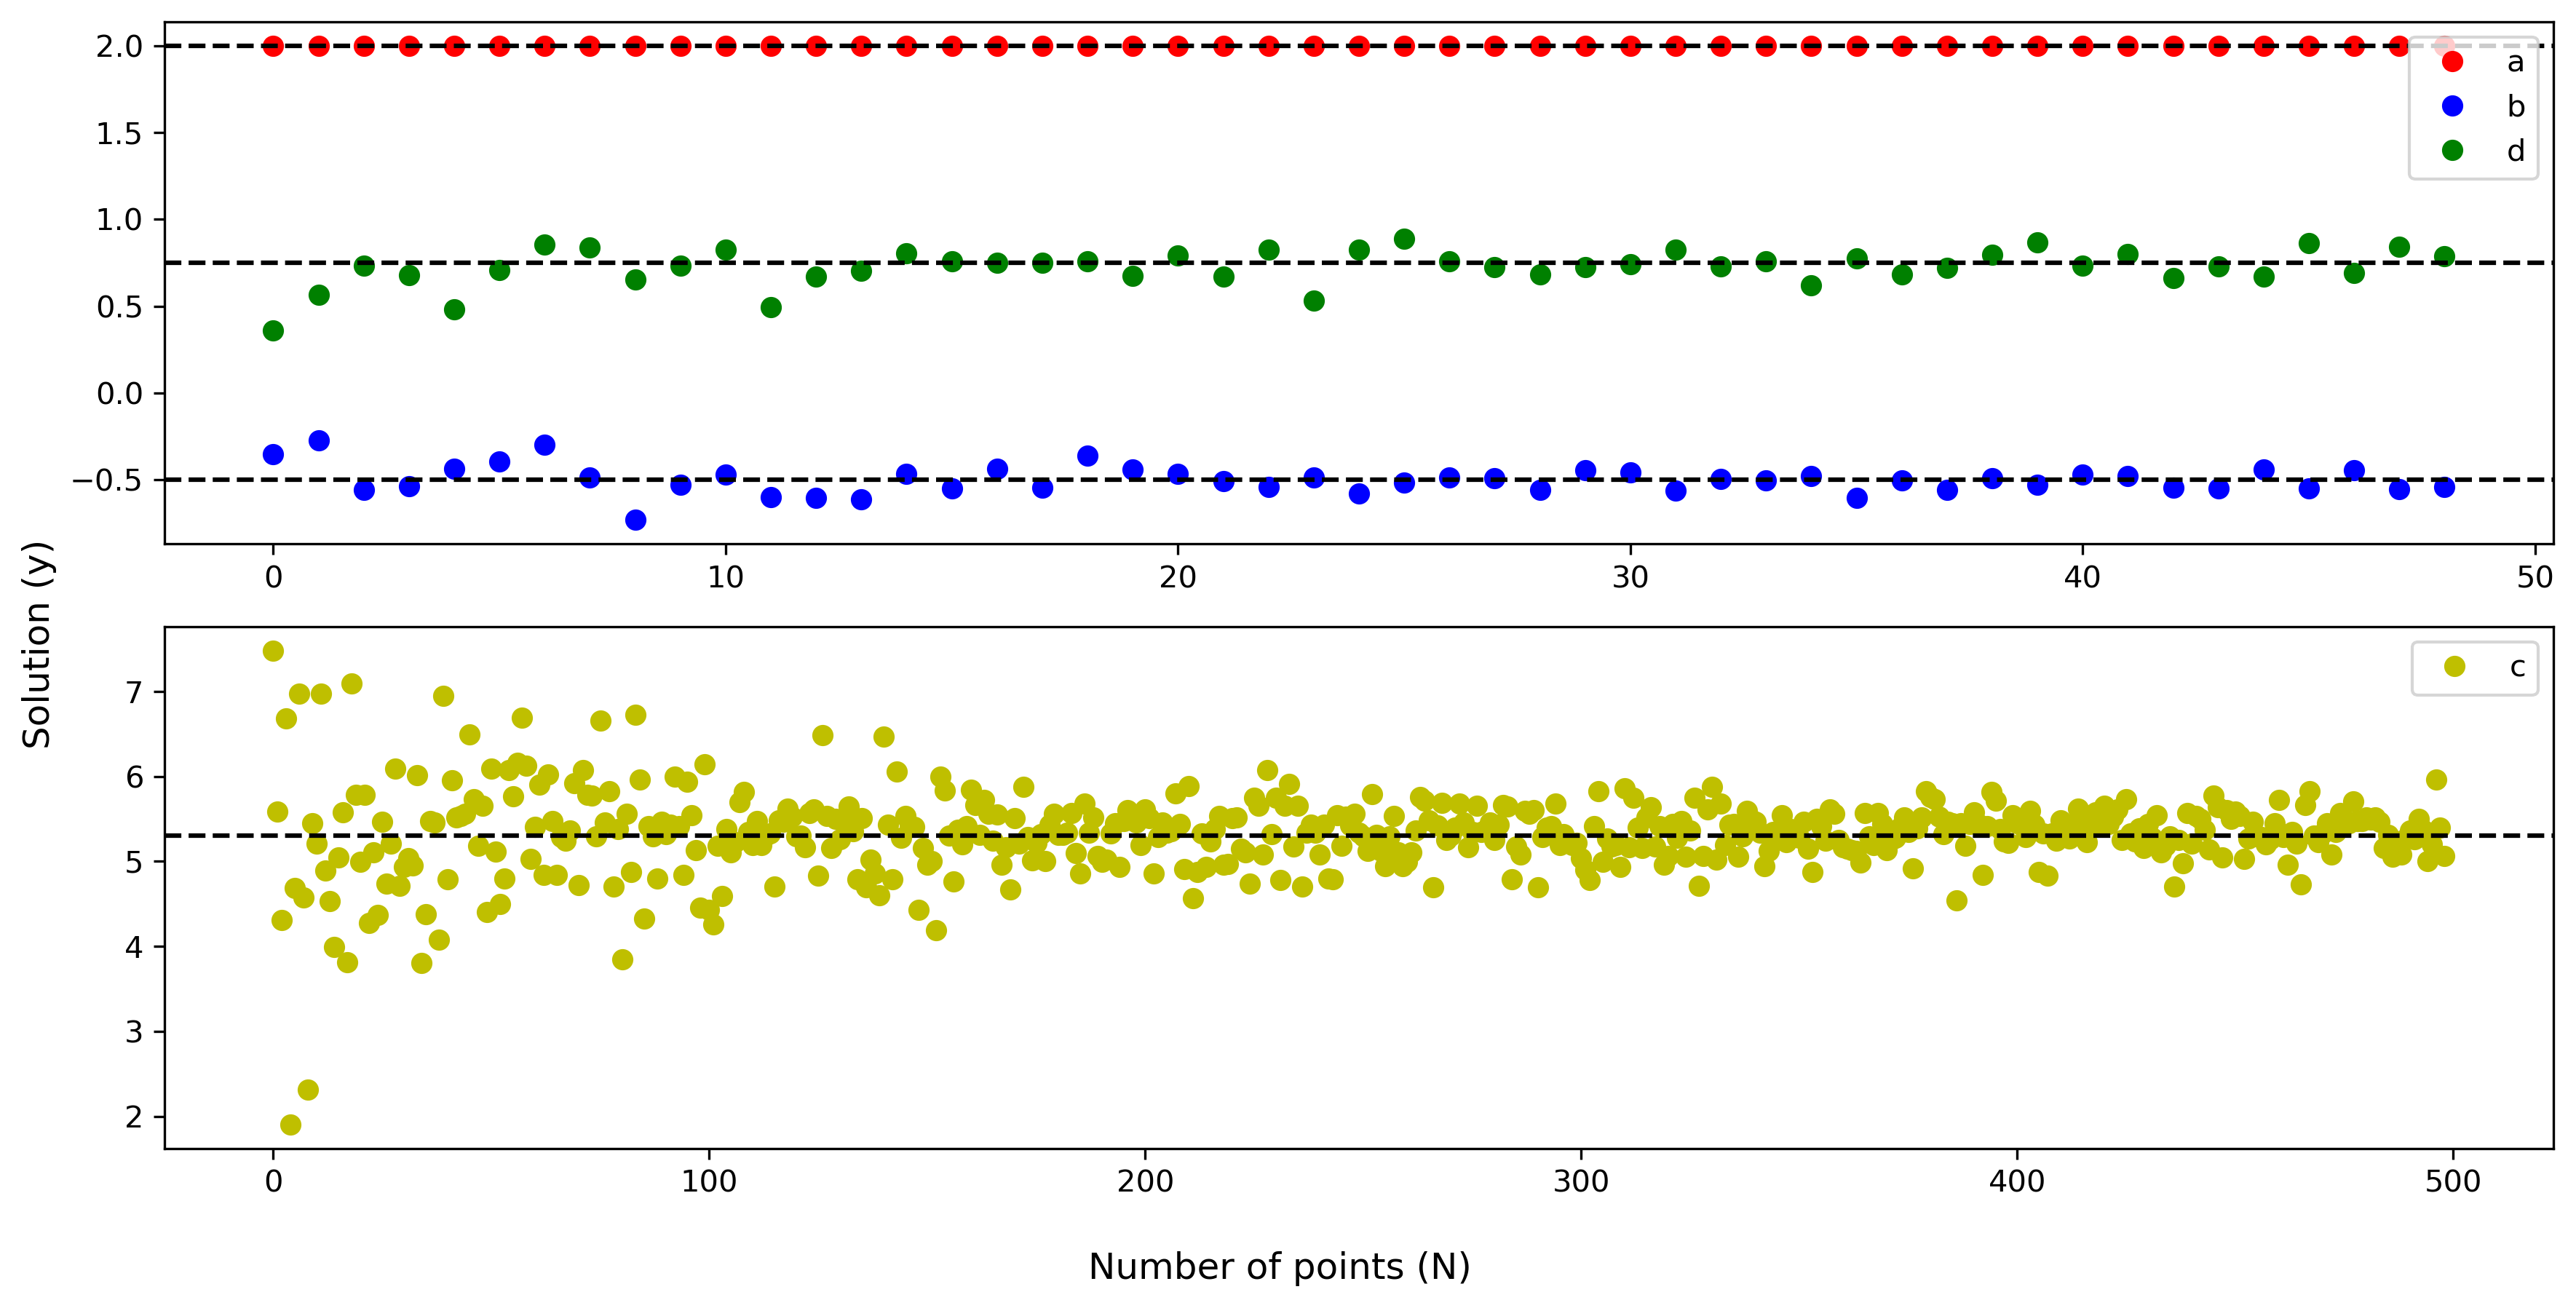
\includegraphics[width=0.8\textwidth]{q-2.png}
    \caption{Solutions to Question 2, black lines are the analytical solutions and the dots are 
    solutions for N number of steps on the monte-carlo integration function. Legend shows the 
    which sub-question the solution points to.}
    \label{fig:q-2}
 \end{figure}

\section{Volume of an n-sphere}
A different function with some similarities to the one in task 1 was written to calculate
the volume of an n-sphere.

\begin{table}[H]
    \centering
    \begin{tabular}{cccc}
    \multicolumn{1}{l}{Radius} & \multicolumn{1}{l}{Dimensions} & \multicolumn{1}{l}{Volume} & \multicolumn{1}{l}{Error} \\
    2.0                          & 3                              & 33.44                      &                           \\
    2.0                          & 5                              & 167.4                      &                          
    \end{tabular}
    \end{table}


\section{9 D Integral}
A jerry rigged attempt was made to calculate the 9D integral. It did not work, there definitely
is an elegant and compact solution but I could'nt figure it out.

\section{Importance sampling with Metropolis Algorithm}

\noindent 
The Metropolis algorithm did not work as required. It was able to generate random
numbers as per given probability distribution shown in the figure below. But 
when trying to use it to find the solution the answer was always wrong. There are 
bugs in the implementation and also a lack of understanding on my part on how to utilise
the generated sample to effectively calculate the solutions. However, the implement 
does seem to work with simple linear functions like f (x) = 2x or f (x) = x +7.

\begin{figure}[H]
    \centering
    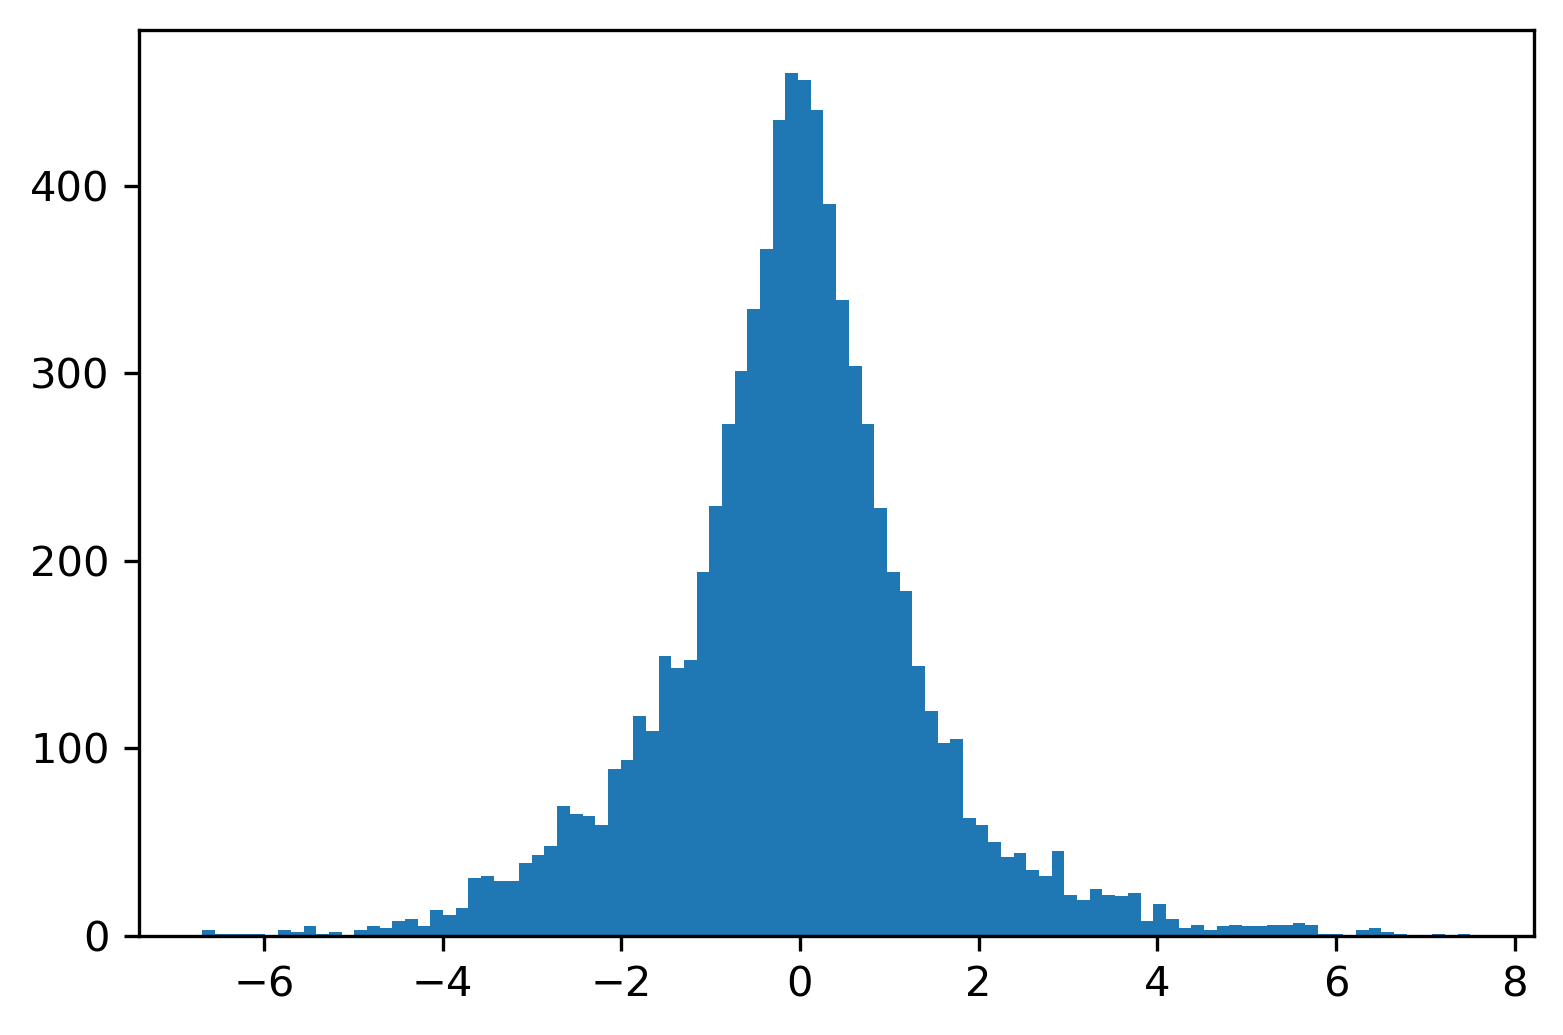
\includegraphics[width=0.45\textwidth]{q-5a.png}
    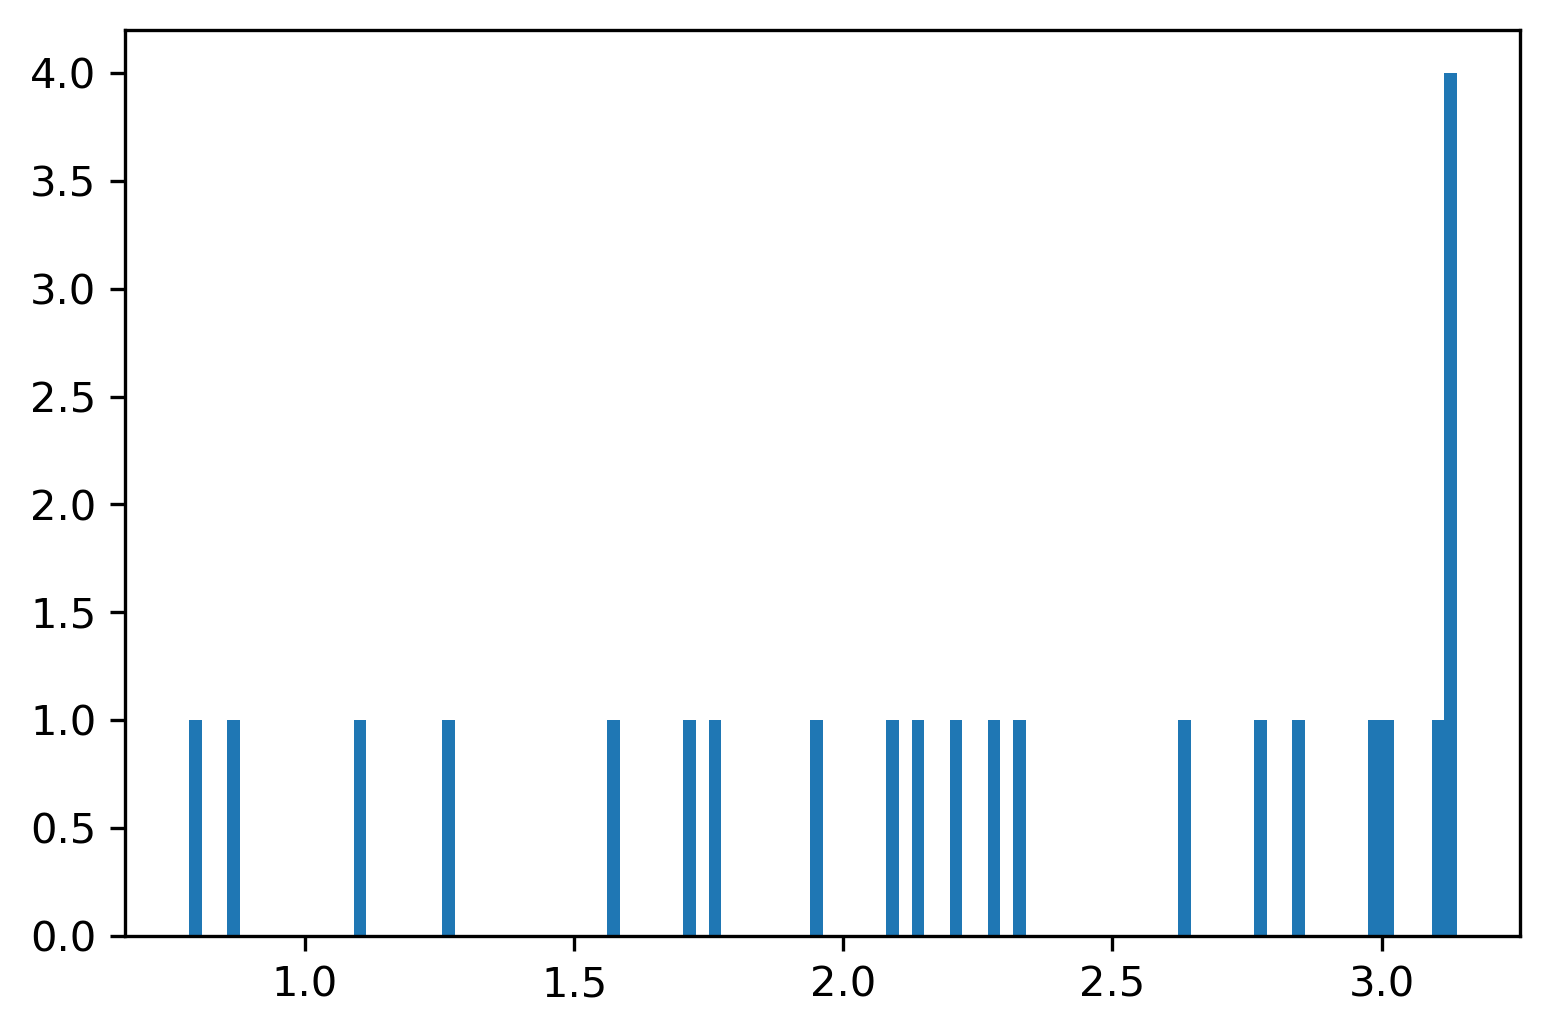
\includegraphics[width=0.45\textwidth]{q-5b.png}
    \caption{Probability distribution of the implementation. The first one for $e^{-|x|}$ looks 
    alright. The other one, not so much. I used $0.1a, 0.1b$ for $\delta$ that worked alright
    for the $e^{-|x|}$ but not well for $sin(x)$.}
    \label{fig:q-5}
 \end{figure}

\section{Uniform sampling comparison with Metropolis Algorithm}

Nothing to compare with cause the implementation does not work well with the functions in the 
question. The following plot shows the convergence of the uniform sampling method. 

\begin{figure}[H]

    \begin{minipage}[c]{0.5\textwidth}
    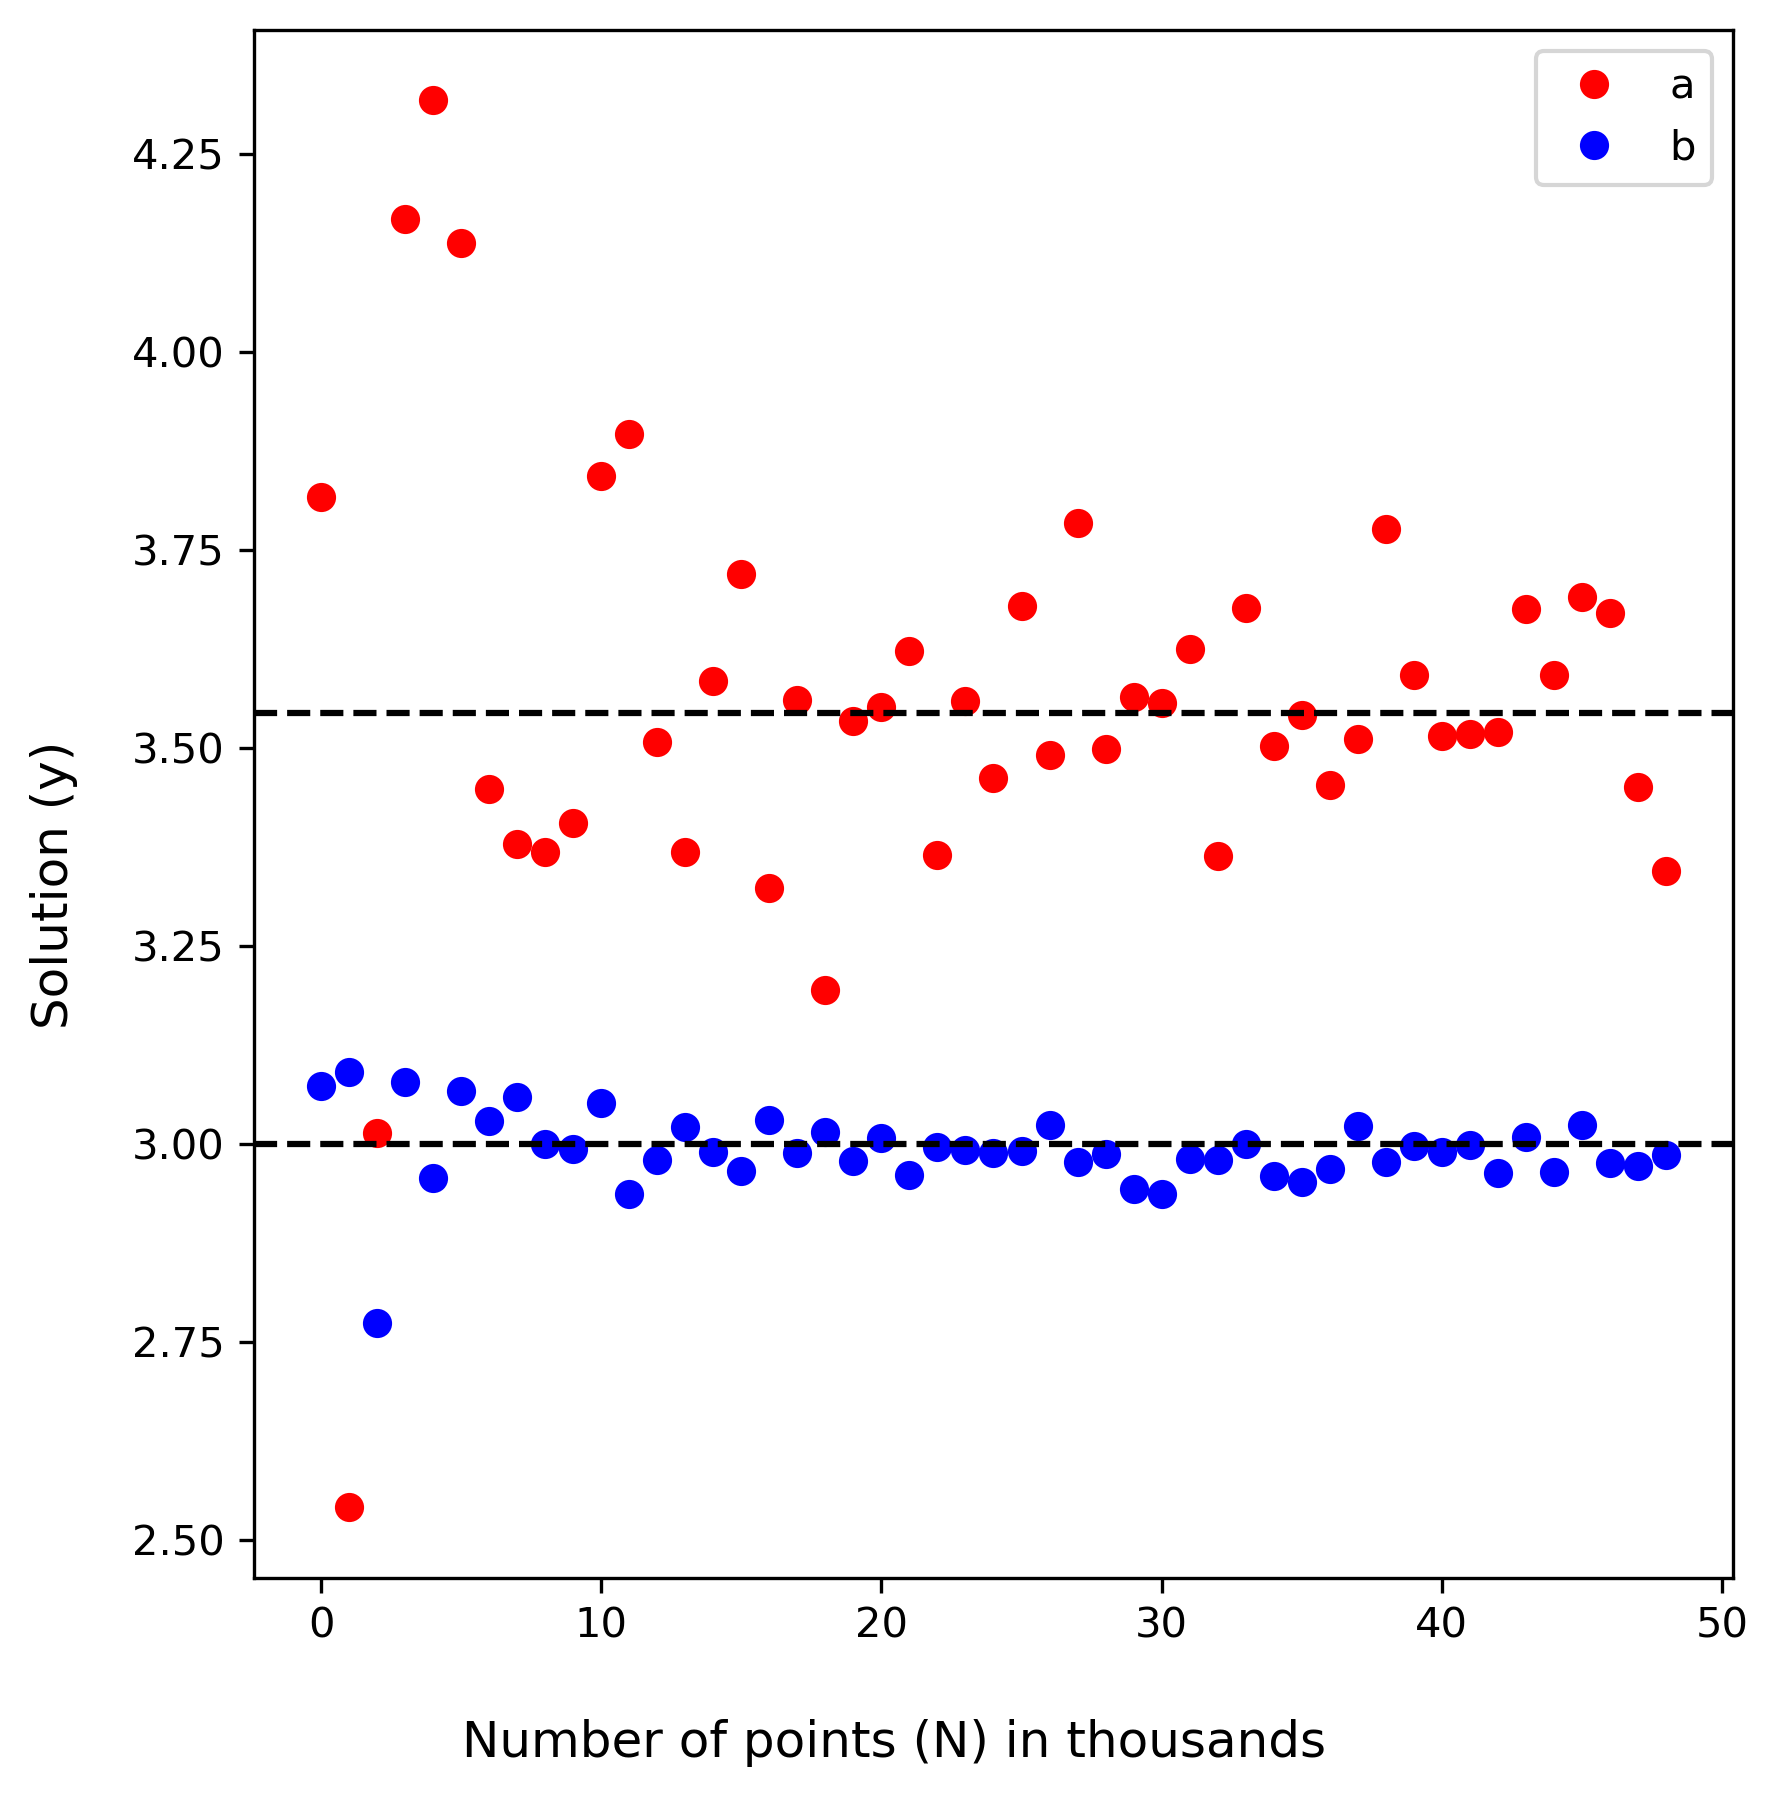
\includegraphics[width=\textwidth]{q-6.png}
    \end{minipage}\hfill
    \begin{minipage}[c]{0.5\textwidth}
    \caption{
        Figure on left shows the convergence of the functions \\
        a) RED : $\int_{-10}^{+10} 2e^{-x^{2}} dx = 3.5360, \\ \\ error = 2.2007e-05 for N = 50000\quad$ \\ \\
        b) BLUE : $\int_{0}^{\pi} 1.5 sin(x) dx = 2.9995 \\ \\ error =2.158e-05 for N = 50000\quad$ \\ \\
        for number of counts N in thousands on x-axis. Function (a) does not 
        converge well and would require a lot more points.
    } \label{fig:task-6}
    \end{minipage}
\end{figure}

\end{document} % This is the end of the document
